\documentclass[10pt, compress]{beamer}

\usetheme{m}

\usepackage{booktabs}
\usepackage[scale=2]{ccicons}
\usepackage{minted}

\usemintedstyle{trac}

\title{Mapping human health risk from \protect\\ contamination of drinking water sources \protect\\ in developing countries}
\subtitle{}
\date{\today}
\author{Avit Kumar Bhowmik}
\institute{Institute for Environmental Sciences, University of Koblenz-Landau \protect\\ \protect\\

\includegraphics[width=0.3\textwidth]{logo.png} \hspace{10pt} 
\includegraphics[width=0.4\textwidth]{logo_conference.png}}

\begin{document}

\maketitle

\begin{frame}%[fragile]
  \frametitle{1/3 of annual mortality in Pakistan is attributed to  \protect\\ contaminated drinking water \small{(Azizullah et al. 2011)}}

  %The \emph{mtheme} is a Beamer theme with minimal visual noise inspired by the
  %\href{https://github.com/hsrmbeamertheme/hsrmbeamertheme}{\textsc{hsrm} Beamer
  %Theme} by Benjamin Weiss.

  %Enable the theme by loading

  %\begin{minted}[fontsize=\small]{latex}
    %\documentclass{beamer}
    %\usetheme{m}
  %\end{minted}

  %Note, that you have to have Mozilla's \emph{Fira Sans} font and XeTeX
  %installed to enjoy this wonderful typography.

  $\vcenter{\hbox{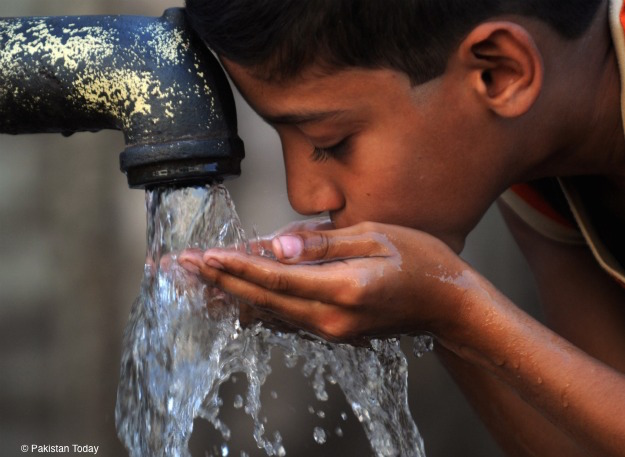
\includegraphics[width=0.32\textwidth]{images/Water_Pakistan.jpg}}}$
  \pause
  \hspace*{10pt}
  $\vcenter{\hbox{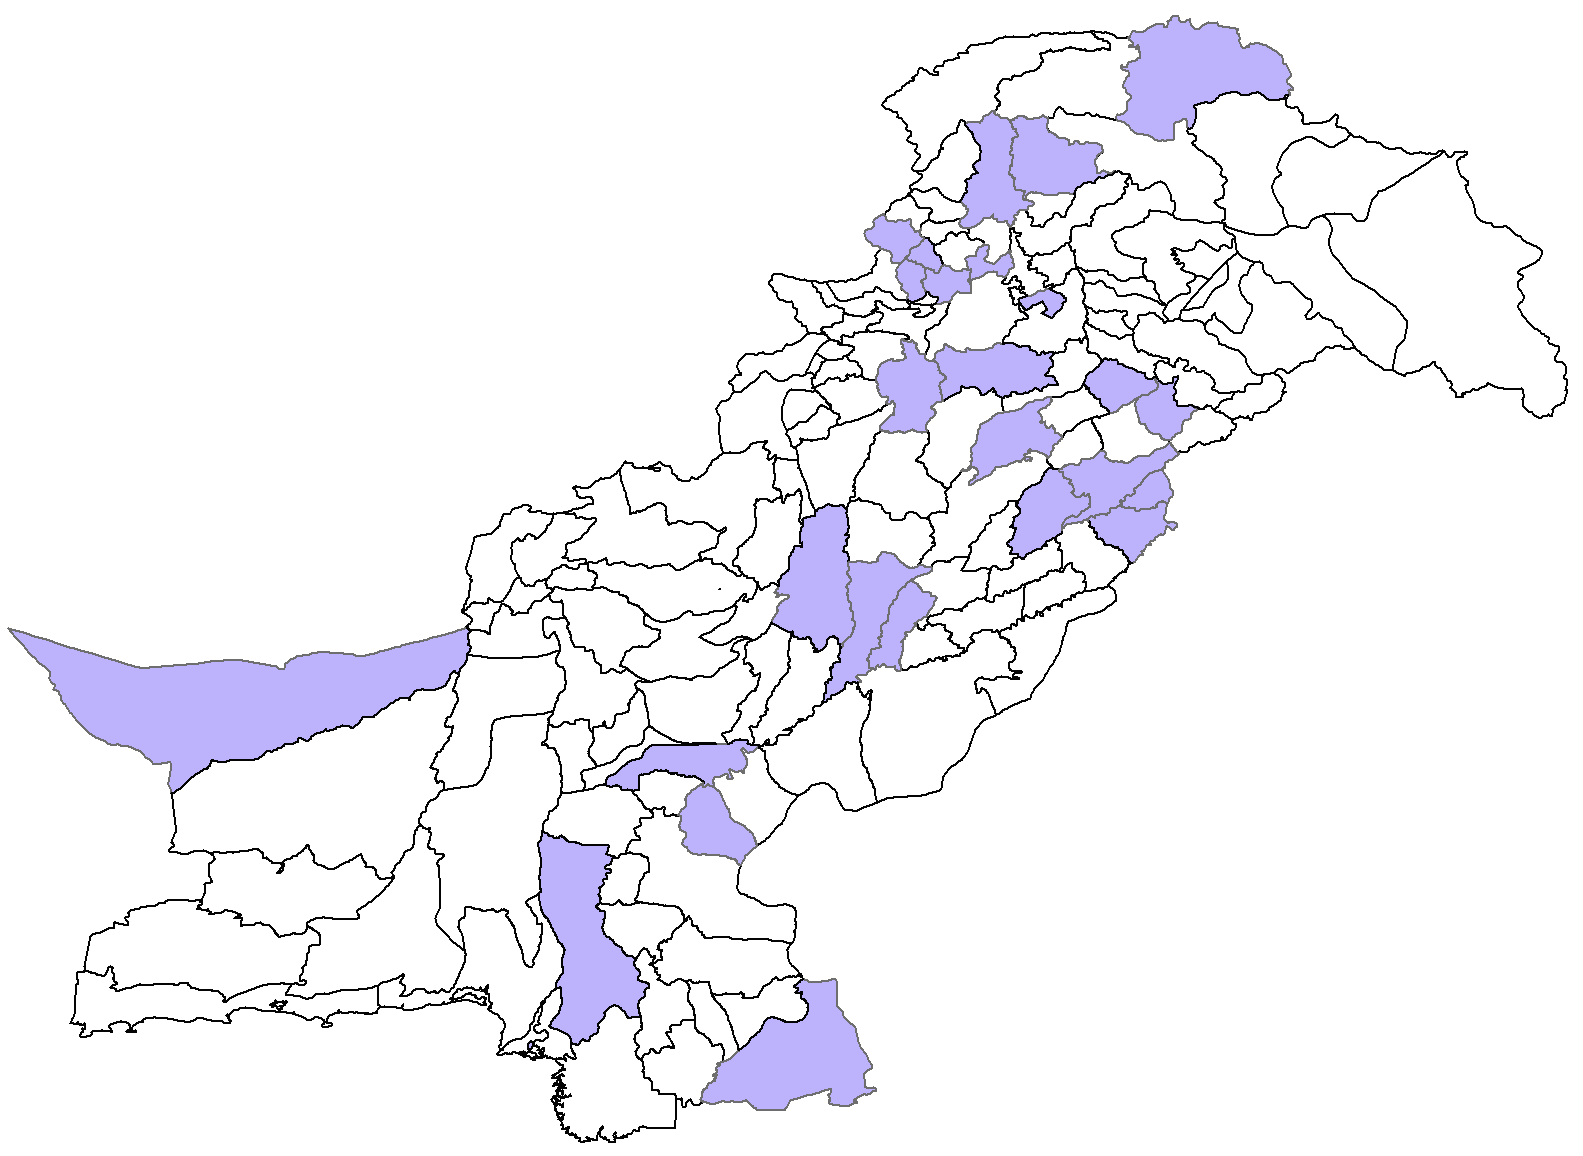
\includegraphics[width=0.62\textwidth]{images/Districts_Pakistan.png}}}$ \\
  \vspace{10pt} \alert{We compiled trace metal concentrations in ground \& surface water} \\
  \pause
  19 \% coverage, max. sampled-unsampled district distance 2000 km \\
  Low global representativeness, GCV $\geq$ 1 \pause \alert{non-stationarity}
\end{frame}

\begin{frame}[fragile]
  \frametitle{Geographically weighted regression (GWR) \protect\\ allows to incorporate local variations \small (Harris et al. 2010)}
  %Sections group slides of the same topic

  %\begin{minted}[fontsize=\small]{latex}
    %\section{Elements}
  %\end{minted}
  %for which the \emph{mtheme} provides a nice progress indicator \ldots
  \begin{equation*}
    C_{T,z} = \delta_{z,0} + \sum_{n=1}^{m=8}\delta_{z,n}S_{z,n} + e_z
    \end{equation*}
    \pause
    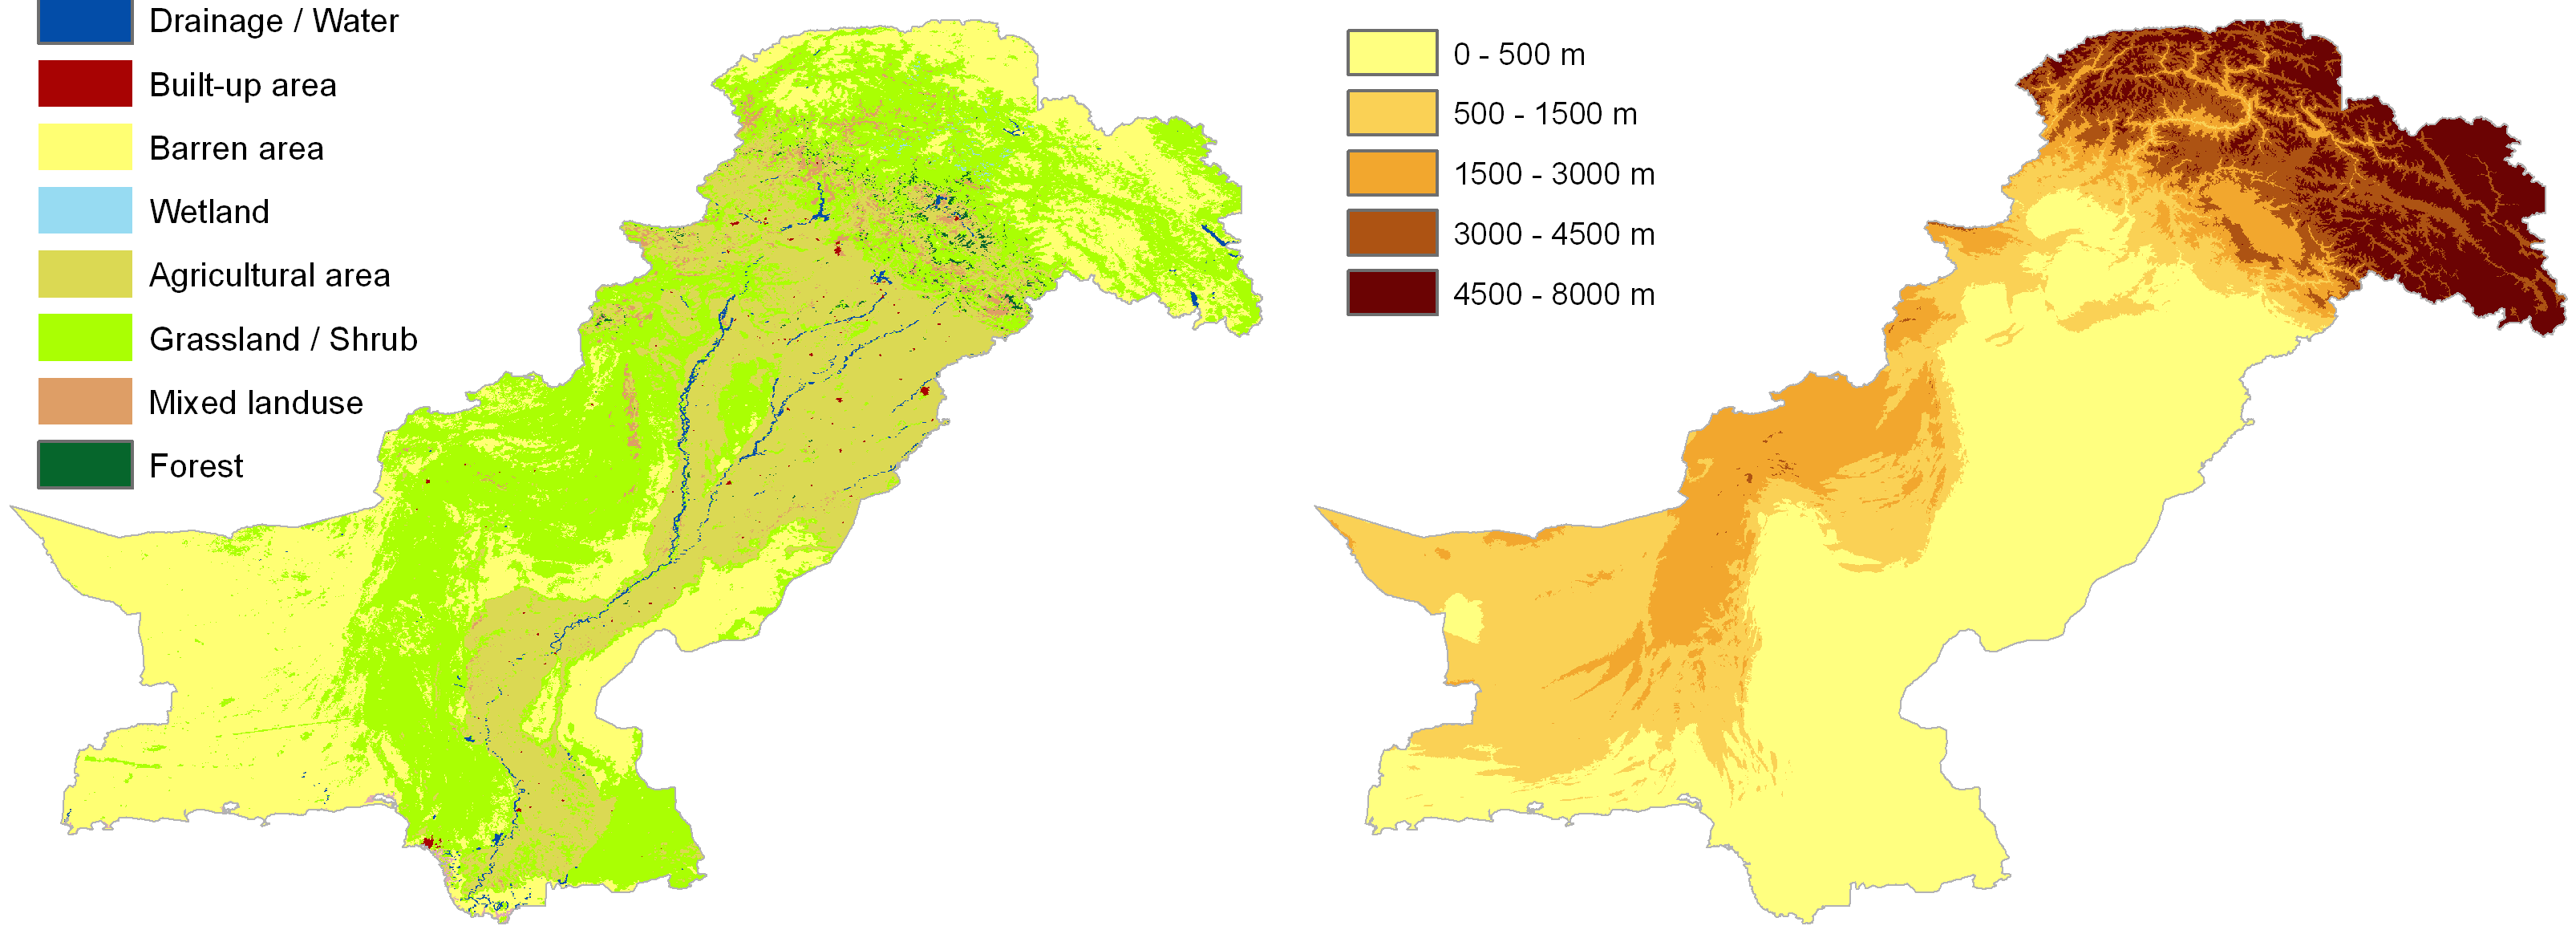
\includegraphics[width=1\textwidth]{images/Spatial_predictors.png} \\
  \alert{Land cover \small{(ISCGM 2014)}} BL, AL, ML \hspace{6pt} \alert{Elevation \small{(Rodriguez et al. 2005)}} \\
  \pause
  \alert{Global soil properties \small{(Batjes 2000)}} SOC, SCC, WC, pH
  
\end{frame}

\begin{frame}[fragile]
  \frametitle{We calibrated local GWR models \protect\\ and used them for spatial prediction}
  %Sections group slides of the same topic

  %\begin{minted}[fontsize=\small]{latex}
    %\section{Elements}
  %\end{minted}
  %for which the \emph{mtheme} provides a nice progress indicator \ldots
  \begin{equation*}
    C_{T,z} = \delta_{z,0} + \sum_{n=1}^{m=8}\delta_{z,n}S_{z,n} + e_z
    \end{equation*}
  \begin{itemize}
        \item \alert{Gaussian kernel} based on the spatial continuity
        \pause
        \item \alert{Fixed kernel bandwidths} based on AIC
        \pause
        \item \alert{Best-fit models} forward entering of spatial predictors and based on AIC \\
        \centering e.g. Cr\_SW\textasciitilde WC + ALU \\
        \pause
        \raggedright
        \item \alert{R package GWmodel} (Gollini et al. 2013)
      \end{itemize}
  
\end{frame}

%\section{Elements}

%\begin{frame}[fragile]
  %\frametitle{Typography}
      %\begin{minted}[fontsize=\small]{latex}
%The theme provides sensible defaults to \emph{emphasis}
%text, \alert{accent} parts or show \textbf{bold} results.
      %\end{minted}

  %\begin{center}becomes\end{center}

  %The theme provides sensible defaults to \emph{emphasis} text,
  %\alert{accent} parts or show \textbf{bold} results.
%\end{frame}

\begin{frame}{We evaluated prediction accuracy and uncertainty by \protect\\ leave-one-out cross-validation}
  %\begin{columns}[onlytextwidth]
    %\column{0.5\textwidth}
      %Items
      \begin{itemize}
        \item \alert{Index of agreement ($d$)} perfect agreement 1, no agreement 0
        \pause
        \item \alert{Root mean squared deviation error ($RMSDE$)} lower value indicates higher accuracy
        \pause
        \item \alert{Standard deviation of prediction z-scores ($SDZ$)} unity indicates high certainty
      \end{itemize}

    %\column{0.5\textwidth}
      %Enumerations
      %\begin{enumerate}
        %\item First, \item Second and \item Last.
      %\end{enumerate}
  %\end{columns}
\end{frame}

\begin{frame}[fragile]
  \frametitle{We estimated area and population at risk \protect\\ by comparing to ``WHO'' guideline thresholds \small{(WHO 2011)}}
  %Sections group slides of the same topic

  %\begin{minted}[fontsize=\small]{latex}
    %\section{Elements}
  %\end{minted}
  %for which the \emph{mtheme} provides a nice progress indicator \ldots
  \centering
  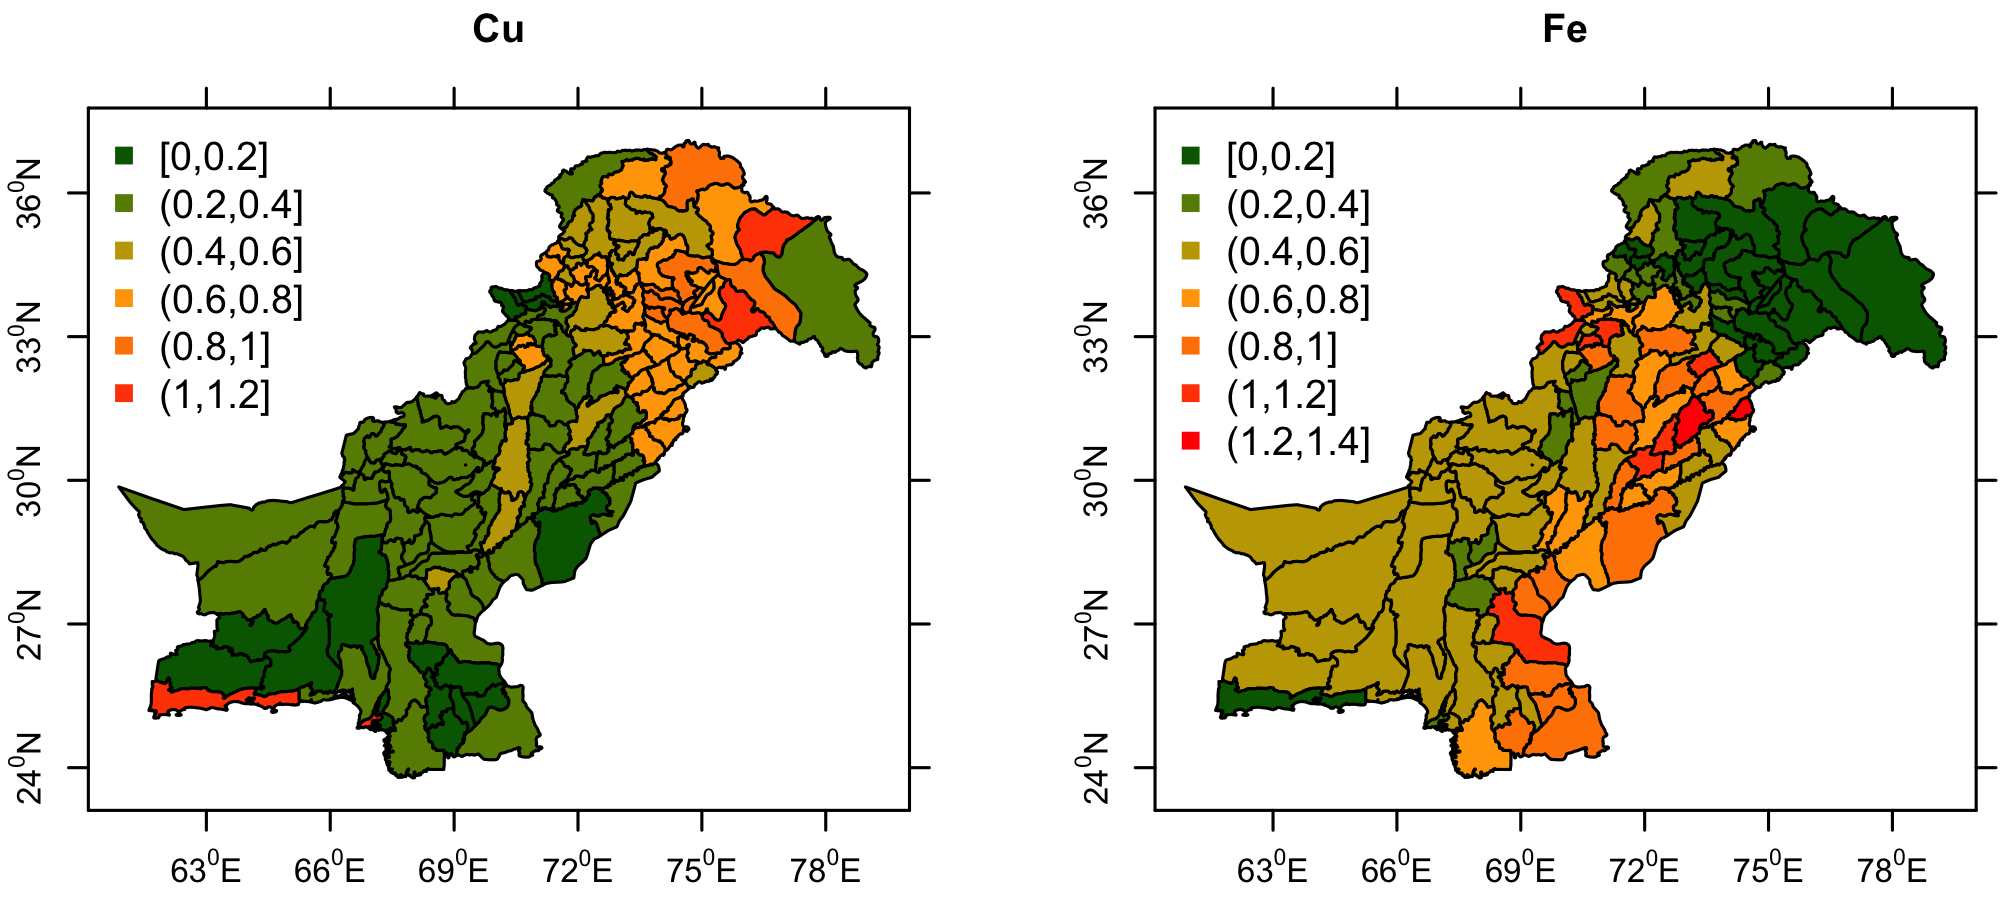
\includegraphics[width=0.9\textwidth]{images/Prediction_example.png}
  \begin{equation*}
    RQ_{T,z} = \frac{\hat{C}_{z,0}}{C_{WHO-T}}
    \end{equation*}
    \pause \\
  \alert{RQ>1} at risk \alert{RQ $\leq$ 1} negligible risk
  
\end{frame}

\begin{frame}[fragile]
  \frametitle{More than 53 \% of total area and 74 million people \protect\\ are at risk from arsenic, chromium, iron, nickel and lead}
  %Sections group slides of the same topic

  %\begin{minted}[fontsize=\small]{latex}
    %\section{Elements}
  %\end{minted}
  %for which the \emph{mtheme} provides a nice progress indicator \ldots
  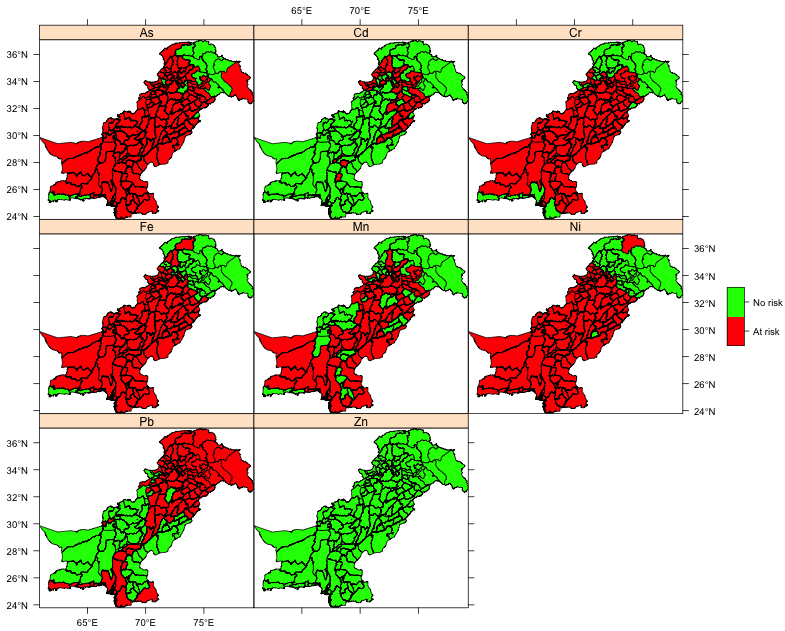
\includegraphics[width=0.88\textwidth]{images/Ground_water_risk.png}
\end{frame}

\begin{frame}[fragile]
  \frametitle{More than 53 \% of total area and 74 million people \protect\\ are at risk from arsenic, chromium, iron, nickel and lead}
  %Sections group slides of the same topic

  %\begin{minted}[fontsize=\small]{latex}
    %\section{Elements}
  %\end{minted}
  %for which the \emph{mtheme} provides a nice progress indicator \ldots
  \centering
  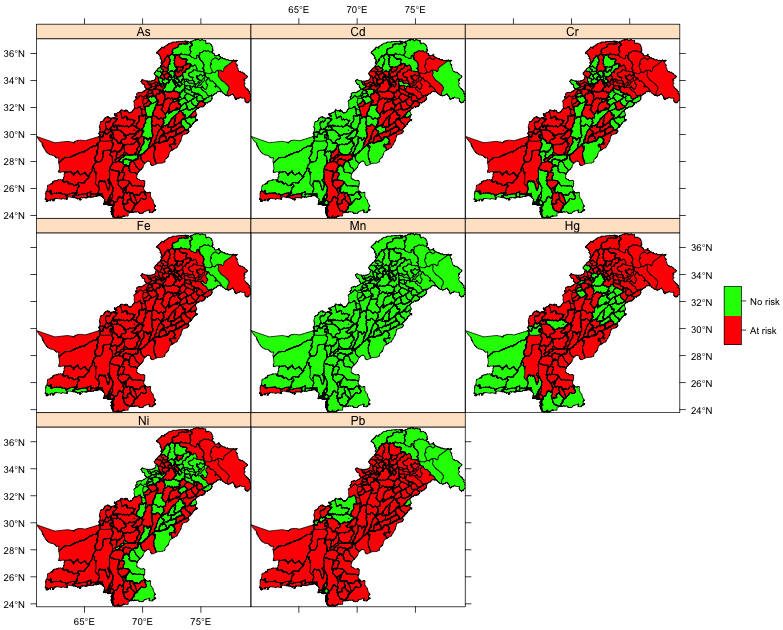
\includegraphics[width=0.88\textwidth]{images/Surface_water_risk.png}
\end{frame}

\begin{frame}{Our GWR model predictions exhibited a high accuracy \protect\\ and a low uncertainty}
  %\begin{columns}[onlytextwidth]
    %\column{0.5\textwidth}
      %Items
      \begin{itemize}
        \item \alert{$d$ \geq 0.8} except for iron in ground water and zinc in surface water
        \pause
        \item \alert{$RMSDE$ \leq 0.45} 0.97 for iron in ground water and 0.8 for zinc in surface water
        \pause
        \item \alert{$SDZ$ \geq 0.7} except for cadmium and zinc in ground water, and cadmium and manganese in surface water
        \pause
        \item \alert{Calibrated spatial predictors are in agreement with the causes of trace metal contamination} e.g. As\_SW\textasciitilde SOC + pH \\ (Husain et al. 2012)
      \end{itemize}
\end{frame}

\begin{frame}{The predictions inform water resources management \protect\\ on potential hot spots}
  %\begin{columns}[onlytextwidth]
    %\column{0.5\textwidth}
      %Items
      \begin{itemize}
        \item \alert{Predictions may not reflect true trace metal concentration variation} 453 km $\leq$ kernel bandwidth $\leq$ 1335 km \\ (Bhowmik and Costa 2014)
        \pause
        \item \alert{Predictions complement field monitoring} although require field validation
        \pause
        \item \alert{Predictions with low accuracy and high uncertainty need to be treated with caution} e.g. zinc
        \pause
        \item \alert{Perhaps over-prediction for areas with access to water purification} more relevant for rural areas (Khan et al. 2012)
        \pause
        \item \alert{May also indicate indirect effects} e.g. via consumption of vegetables irrigated with contaminated water (Amin et al., 2012)
      \end{itemize}
\end{frame}

%\begin{frame}{Descriptions}
  %\begin{description}
    %\item[PowerPoint] Meeh.
    %\item[Beamer] Yeeeha.
  %\end{description}
%\end{frame}
%\begin{frame}{Animation}
  %\begin{itemize}[<+- | alert@+>]
    %\item \alert<4>{This is\only<4>{ really} important}
    %\item Now this
    %\item And now this
  %\end{itemize}
%\end{frame}

%\begin{frame}{Figures}
  %\begin{figure}
    %\newcounter{density}
    %\setcounter{density}{20}
    %\begin{tikzpicture}
      %\def\couleur{mLightBrown}
      %\path[coordinate] (0,0)  coordinate(A)
       %           ++( 90:5cm) coordinate(B)
        %          ++(0:5cm) coordinate(C)
         %         ++(-90:5cm) coordinate(D);
      %\draw[fill=\couleur!\thedensity] (A) -- (B) -- (C) --(D) -- cycle;
      %\foreach \x in {1,...,40}{%
          %\pgfmathsetcounter{density}{\thedensity+20}
          %\setcounter{density}{\thedensity}
          %\path[coordinate] coordinate(X) at (A){};
          %\path[coordinate] (A) -- (B) coordinate[pos=.10](A)
           %                   -- (C) coordinate[pos=.10](B)
            %                  -- (D) coordinate[pos=.10](C)
             %                 -- (X) coordinate[pos=.10](D);
          %\draw[fill=\couleur!\thedensity] (A)--(B)--(C)-- (D) -- cycle;
      %}
    %\end{tikzpicture}
    %\caption{Rotated square from
    %\href{http://www.texample.net/tikz/examples/rotated-polygons/}{texample.net}.}
  %\end{figure}
%\end{frame}
%\begin{frame}{Tables}
  %\begin{table}
    %\caption{Largest cities in the world (source: Wikipedia)}
    %\begin{tabular}{lr}
      %\toprule
      %City & Population\\
      %\midrule
      %Mexico City & 20,116,842\\
      %Shanghai & 19,210,000\\
      %Peking & 15,796,450\\
      %Istanbul & 14,160,467\\
      %\bottomrule
    %\end{tabular}
  %\end{table}
%\end{frame}
%\begin{frame}{Blocks}

  %\begin{block}{This is a block title}
    %This is soothing.
  %\end{block}

%\end{frame}
%\begin{frame}{Math}
  %\begin{equation*}
    %e = \lim_{n\to \infty} \left(1 + \frac{1}{n}\right)^n
  %\end{equation*}
%\end{frame}
%\begin{frame}{Quotes}
  %\begin{quote}
    %Veni, Vidi, Vici
  %\end{quote}
%\end{frame}

%\plain{Dark background}{\vspace{-2em}\begin{center}\includegraphics[width=\textwidth]{images/valley.jpg}\end{center}}

%\section{Conclusion}

%\begin{frame}{Summary}

  %Get the source of this theme and the demo presentation from

  %\begin{center}\url{github.com/matze/mtheme}\end{center}

  %The theme \emph{itself} is licensed under a
  %\href{http://creativecommons.org/licenses/by-sa/4.0/}{Creative Commons
  %Attribution-ShareAlike 4.0 International License}.

  %\begin{center}\ccbysa\end{center}

%\end{frame}

\plain{}{\small{For more: Bhowmik et al. 2015, Sci. Tot. Env. \textit{under review}} \\
\vspace{5pt} Collaborators: Ambreen Alamdar, Ioannis Katsoyiannis, Heqing Shen, Nadeem Ali, Syeda Maria Ali, Habib Bokhari, Ralf B. Schäfer, \\ Syed Ali Musstjab Akber Shah Eqani \\
\vspace{20pt} \LARGE{Thank you} \\ \vspace{20pt} Questions?}

\end{document}
